\documentclass[12pt,a4paper]{article}
\usepackage[a4paper, margin=0.8in, headheight=14pt]{geometry}
\usepackage{fontspec}
\usepackage{unicode-math}
\setmainfont{TeX Gyre Pagella}
\setmonofont[Scale=0.88]{TeX Gyre Cursor}
\setmathfont{Latin Modern Math}

\usepackage{xcolor}
\usepackage{colortbl}
\usepackage{titlesec}
\usepackage{enumitem}
\usepackage{tabularx}
\usepackage{booktabs}
\usepackage{array}
\usepackage{amsmath}
\allowdisplaybreaks
\usepackage{tikz}
\usetikzlibrary{shapes.geometric, arrows.meta, positioning, calc, fit, decorations.pathreplacing, patterns}
\usepackage{tcolorbox}
\tcbuselibrary{skins, breakable}
\usepackage{hyperref}
\usepackage{fancyhdr}
\usepackage{graphicx}
\usepackage{microtype}
\hyphenpenalty=10000
\exhyphenpenalty=10000
\sloppy
\usepackage{caption}
\usepackage{setspace}
\usepackage{multirow}
\usepackage{tocloft}

% ─── Q&A helper ────────────────────────────────────────────────────────────────
\newcommand{\Q}[1]{\textbf{#1}\par\noindent\ignorespaces}

% ─── Colour Palette ────────────────────────────────────────────────────────────
\definecolor{myred}{RGB}{196,30,58}
\definecolor{mydark}{RGB}{30,30,50}
\definecolor{mygreen}{RGB}{14,120,80}
\definecolor{myteal}{RGB}{0,130,140}
\definecolor{myamber}{RGB}{220,130,20}
\definecolor{mypurple}{RGB}{90,40,140}
\definecolor{mygray}{RGB}{248,249,251}
\definecolor{mgframe}{RGB}{215,220,230}
\definecolor{watermark}{RGB}{145,150,170}
\definecolor{hdrred}{RGB}{250,232,235}
\definecolor{hdrgreen}{RGB}{220,244,233}
\definecolor{hdrteal}{RGB}{220,242,244}
\definecolor{hdramber}{RGB}{253,242,215}
\definecolor{hdrpurple}{RGB}{238,228,255}
\definecolor{hdrgray}{RGB}{238,240,245}
\definecolor{rowalt}{RGB}{250,251,253}

% ─── Section Formatting ────────────────────────────────────────────────────────
\titleformat{\section}
  {\large\bfseries\color{myred}}{\thesection.}{0.5em}{}
  [\vspace{1pt}{\color{myred}\rule{\linewidth}{0.8pt}}]
\titleformat{\subsection}
  {\normalsize\bfseries\color{myteal}}{\thesubsection}{0.5em}{}
\titlespacing*{\section}{0pt}{18pt}{7pt}
\titlespacing*{\subsection}{0pt}{11pt}{4pt}

% ─── Paragraph ─────────────────────────────────────────────────────────────────
\setlength{\parindent}{0pt}
\setlength{\parskip}{4pt}

% ─── TOC Styling ───────────────────────────────────────────────────────────────
\renewcommand{\cfttoctitlefont}{\large\bfseries\color{myred}}
\renewcommand{\cftaftertoctitle}{\par\noindent{\color{myred}\rule{\linewidth}{0.8pt}}}
\setlength{\cftbeforetoctitleskip}{0pt}
\setlength{\cftaftertoctitleskip}{6pt}
\renewcommand{\cftsecfont}{\normalsize\bfseries\color{mydark}}
\renewcommand{\cftsecpagefont}{\normalsize\bfseries\color{mydark}}
\renewcommand{\cftsecleader}{\cftdotfill{\cftdotsep}}
\setlength{\cftbeforesecskip}{7pt}
\renewcommand{\cftsubsecfont}{\small\color{mydark}}
\renewcommand{\cftsubsecpagefont}{\small\color{mydark}}
\setlength{\cftbeforesubsecskip}{3pt}
\setlength{\cftsubsecindent}{1.4em}

% ─── Table helpers ─────────────────────────────────────────────────────────────
\renewcommand{\arraystretch}{1.45}
\setlength{\tabcolsep}{6pt}
\arrayrulecolor{mydark}
\newcolumntype{B}[1]{>{\small\bfseries\raggedright\arraybackslash}m{#1}}
\newcolumntype{Y}{>{\small\raggedright\arraybackslash}X}
\renewcommand{\tabularxcolumn}[1]{m{#1}}

% ─── Header / Footer ───────────────────────────────────────────────────────────
\pagestyle{fancy}
\fancyhf{}
\fancyhead[L]{\small\color{myred}\textbf{EC303}\;\color{mydark}--- Signals and System}
\fancyhead[R]{\small\color{myteal}\textbf{Module 1 Notes}}
\fancyfoot[C]{\small\color{mydark}\thepage}
\fancyfoot[R]{\small\color{watermark}\textit{\copyright\ Biraj}}
\renewcommand{\headrulewidth}{0.5pt}
\renewcommand{\footrulewidth}{0.3pt}

% ─── Hyperref ──────────────────────────────────────────────────────────────────
\hypersetup{
  colorlinks=true, linkcolor=myteal, urlcolor=myteal,
  pdfauthor={Biraj Sarkar (CGEC)},
  pdftitle={EC303 --- Module 1 Notes: Introduction to Signals and Systems}
}

% ─── tcolorbox styles ──────────────────────────────────────────────────────────
\tcbset{
  tikzbox/.style={
    colback=mygray, colframe=mgframe, boxrule=0.6pt, arc=4pt,
    left=8pt, right=8pt, top=6pt, bottom=6pt,
    colbacktitle=mgframe, coltitle=mydark,
    fonttitle=\small\bfseries
  },
  defbox/.style={
    colback=hdrgreen, colframe=mygreen, boxrule=0.8pt, arc=4pt,
    left=9pt, right=9pt, top=6pt, bottom=6pt,
    colbacktitle=mygreen, coltitle=white,
    fonttitle=\small\bfseries
  },
  formulabox/.style={
    colback=hdrteal, colframe=myteal, boxrule=0.8pt, arc=4pt,
    left=9pt, right=9pt, top=6pt, bottom=6pt,
    colbacktitle=myteal, coltitle=white,
    fonttitle=\small\bfseries
  },
  examplebox/.style={
    colback=hdramber, colframe=myamber, boxrule=0.8pt, arc=4pt,
    left=9pt, right=9pt, top=6pt, bottom=6pt,
    colbacktitle=myamber, coltitle=white,
    fonttitle=\small\bfseries
  },
  masonbox/.style={
    colback=hdrpurple, colframe=mypurple, boxrule=0.8pt, arc=4pt,
    left=9pt, right=9pt, top=6pt, bottom=6pt,
    colbacktitle=mypurple, coltitle=white,
    fonttitle=\small\bfseries
  },
  exambox/.style={
    colback=hdrpurple, colframe=mypurple, boxrule=1pt, arc=5pt,
    left=10pt, right=10pt, top=8pt, bottom=8pt,
    colbacktitle=mypurple, coltitle=white,
    fonttitle=\bfseries,
    breakable, title after break={\textbf{Frequently Asked / Viva Questions (contd.)}}
  }
}

\tcbset{breakable}
\tcbset{after={\color{black}}}

% ─── TikZ styles ───────────────────────────────────────────────────────────────
\tikzset{
  sysblock/.style={rectangle, draw=myteal, fill=hdrteal,
    minimum width=2.4cm, minimum height=1.1cm,
    font=\small\bfseries, rounded corners=3pt, line width=0.8pt, align=center},
  sigarrow/.style={-Stealth, thick, color=mydark},
  sigcircle/.style={circle, draw=myred, fill=hdrred, inner sep=2pt, font=\small\bfseries}
}

\begin{document}

% ─── Title Page ───────────────────────────────────────────────────────────────
\begin{center}
  {\LARGE\bfseries\color{myred} EC303 --- Signals and System}\\[5pt]
  {\normalsize\color{mydark} Semester III \quad$\bullet$\quad 3L:0T:0P \quad$\bullet$\quad 3 Credits}\\[3pt]
  {\normalsize\color{myteal}\textbf{Module 1 Exam Notes: Signal Classifications, Elementary Signals \& System Properties}}\\[3pt]
  {\small\color{mydark} CGEC \;$|$\; B.Tech ECE (2023--27) \;$|$\; \textit{Biraj Sarkar}}
\end{center}
\vspace{2pt}
\noindent{\color{myred}\rule{\linewidth}{1.5pt}}
\vspace{2pt}

\hypersetup{linkcolor=mydark}
\tableofcontents
\hypersetup{linkcolor=myteal}
\newpage

% ===============================================================================
\section{Signals and Systems in Engineering and Science}
% ===============================================================================

\subsection{Basic Definitions}
\begin{tcolorbox}[defbox, title={\textbf{Definition: Signal and System}}]
\begin{itemize}[leftmargin=*, itemsep=4pt]
  \item \textbf{Signal:} A physical quantity that varies with one or more independent variables (such as time $t$, spatial coordinates $x, y, z$, or frequency $\omega$) and conveys information regarding the state or behavior of a physical phenomenon. Mathematically, a signal is represented as a single-valued function of independent variable(s), e.g., voltage $v(t)$, acoustic pressure $p(t)$, or pixel intensity matrix $I(x,y)$.
  \item \textbf{System:} An interconnection of physical components, mathematical operators, or software algorithms that accepts an excitation/input signal $x(t)$ or $x[n]$ and produces a corresponding response/output signal $y(t)$ or $y[n]$ according to a well-defined transformation rule:
  \begin{equation}
    y(t) = \mathcal{T}\{x(t)\} \quad \text{or} \quad y[n] = \mathcal{T}\{x[n]\}
  \end{equation}
\end{itemize}
\end{tcolorbox}

\subsection{Real-World Engineering and Scientific Applications}
\begin{itemize}[leftmargin=*, itemsep=3pt]
  \item \textbf{Biomedical Engineering:} Electrocardiogram (ECG) capturing cardiac electrical dipole potentials; Electroencephalogram (EEG) recording neuro-electrical cortical oscillations; photoplethysmogram (PPG) sensing arterial blood volume changes.
  \item \textbf{Telecommunication Systems:} Radio-frequency (RF) modulated electromagnetic waves transmitting digitized speech, video bitstreams, and satellite downlink carrier signals through multipath fading channels.
  \item \textbf{Control and Automation:} Robotic arm angular position feedback sensed by optical encoders; cruise control velocity tracking loops; chemical process temperature/pressure control systems.
  \item \textbf{Geophysics and Seismology:} Primary ($P$) and secondary ($S$) acoustic shear waves recorded by three-axis seismographs for earthquake hypocenter localization and subterranean hydrocarbon reservoir mapping.
  \item \textbf{Speech and Acoustic Processing:} Continuous-time acoustic pressure variations captured by microphones, filtered through anti-aliasing networks, and converted into discrete speech feature vectors for automated speech recognition.
\end{itemize}

\begin{tcolorbox}[tikzbox, title={\textbf{General Input-Output System Architecture}}]
\begin{center}
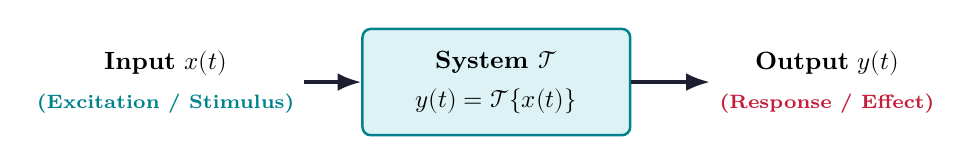
\begin{tikzpicture}[>=Latex, font=\small]
  % Input Node
  \node[align=center] (in) at (-4.2, 0) {
    \textbf{Input} $x(t)$\\[3pt]
    {\scriptsize\color{myteal}\textbf{(Excitation / Stimulus)}}
  };

  % Central System Block
  \node[sysblock, minimum width=3.4cm, minimum height=1.35cm, line width=0.9pt, align=center] (sys) at (0, 0) {
    \textbf{System} $\boldsymbol{\mathcal{T}}$\\[3pt]
    $y(t) = \mathcal{T}\{x(t)\}$
  };

  % Output Node
  \node[align=center] (out) at (4.2, 0) {
    \textbf{Output} $y(t)$\\[3pt]
    {\scriptsize\color{myred}\textbf{(Response / Effect)}}
  };

  % Connecting Arrows with ample clearance
  \draw[->, very thick, color=mydark, -{Latex[length=3mm]}] (in.east) -- (sys.west);
  \draw[->, very thick, color=mydark, -{Latex[length=3mm]}] (sys.east) -- (out.west);
\end{tikzpicture}
\end{center}
\end{tcolorbox}

% ===============================================================================
\section{Classification of Signals}
% ===============================================================================

Signals are classified based on the continuity of their independent variable (time) and dependent variable (amplitude), their periodicity, symmetry, and energy/power distribution.

\subsection{Continuous-Time (CT) vs. Discrete-Time (DT) Signals}
\begin{itemize}[leftmargin=*, itemsep=3pt]
  \item \textbf{Continuous-Time (CT) Signals:} The independent variable $t$ is continuous and defined across an uncountable continuum of real numbers ($t \in \mathbb{R}$). Represented mathematically as $x(t)$.
  \item \textbf{Discrete-Time (DT) Signals:} The independent variable $n$ is defined strictly at discrete integer index points ($n \in \mathbb{Z}$). Often generated by sampling an underlying CT signal at uniform sampling intervals $T_s$, such that $x[n] = x(n T_s)$.
\end{itemize}

\subsection{Continuous-Amplitude vs. Discrete-Amplitude Signals}
\begin{itemize}[leftmargin=*, itemsep=3pt]
  \item \textbf{Continuous-Amplitude Signals (Analog Signals):} The signal amplitude can assume any arbitrary value within a continuous dynamic range $[V_{\min}, V_{\max}]$.
  \item \textbf{Discrete-Amplitude Signals (Quantized / Digital Signals):} The signal amplitude is constrained to a finite, discrete set of predetermined quantization levels $L = 2^b$, where $b$ is the number of encoding bits.
\end{itemize}

\subsection{Periodic vs. Aperiodic Signals}
\begin{tcolorbox}[defbox, title={\textbf{Periodicity Criteria in Continuous and Discrete Time}}]
\begin{itemize}[leftmargin=*, itemsep=4pt]
  \item \textbf{Continuous-Time Periodicity:} A signal $x(t)$ is periodic if there exists a positive non-zero constant $T_0 > 0$ such that:
  \begin{equation}
    x(t + T_0) = x(t) \quad \forall t \in \mathbb{R}
  \end{equation}
  The smallest such positive value $T_0$ is the \textbf{fundamental period} (in seconds), with fundamental angular frequency $\omega_0 = \frac{2\pi}{T_0}$ (rad/s) and cyclic frequency $f_0 = \frac{1}{T_0}$ (Hz).
  \item \textbf{Discrete-Time Periodicity (Critical Difference):} A discrete-time sequence $x[n]$ is periodic if there exists an integer $N > 0$ such that:
  \begin{equation}
    x[n + N] = x[n] \quad \forall n \in \mathbb{Z}
  \end{equation}
  \textbf{Necessary and Sufficient Condition for DT Sinusoid Periodicity:} For $x[n] = \cos(\omega_0 n + \phi)$ or $e^{j\omega_0 n}$ to be periodic, the ratio of its angular frequency to $2\pi$ must be a strictly \textbf{rational number}:
  \begin{equation}
    \frac{\omega_0}{2\pi} = \frac{m}{N} \implies N = m \left(\frac{2\pi}{\omega_0}\right) \in \mathbb{Z}^+
  \end{equation}
  where $m, N$ are coprime integers. If $\omega_0 / 2\pi$ is irrational (e.g., $\omega_0 = 1$ rad), the DT sinusoid is strictly \textbf{aperiodic}.
\end{itemize}
\end{tcolorbox}

\begin{tcolorbox}[examplebox, title={\textbf{Example: Sum of Periodic Signals in CT vs. DT}}]
\textbf{Case 1 (CT):} $x(t) = \cos\left(\frac{\pi}{3}t\right) + \sin\left(\frac{\pi}{4}t\right)$.
Periods: $T_1 = \frac{2\pi}{\pi/3} = 6\text{ s}$, $T_2 = \frac{2\pi}{\pi/4} = 8\text{ s}$.
Ratio: $\frac{T_1}{T_2} = \frac{6}{8} = \frac{3}{4} \in \mathbb{Q}$ (Rational).
Overall fundamental period $T_0 = \text{LCM}(T_1, T_2) = \text{LCM}(6, 8) = 24\text{ s}$. The sum is \textbf{periodic}.

\textbf{Case 2 (DT):} $x[n] = \cos\left(\frac{3\pi}{7}n\right) + \sin\left(\frac{\pi}{5}n\right)$.
$N_1 = \frac{2\pi(7)}{3\pi} = \frac{14}{3} \implies N_1 = 14$ (for $m=3$).
$N_2 = \frac{2\pi(5)}{\pi} = 10$ (for $m=1$).
Overall period $N_0 = \text{LCM}(14, 10) = 70$ samples. The sum is \textbf{periodic}.
\end{tcolorbox}

\subsection{Even (Symmetric) and Odd (Antisymmetric) Signals}
Every arbitrary signal $x(t)$ can be decomposed uniquely into a sum of an even component $x_e(t)$ and an odd component $x_o(t)$:
\begin{equation}
  x(t) = x_e(t) + x_o(t)
\end{equation}
where:
\begin{equation}
  x_e(t) = \frac{x(t) + x(-t)}{2} = x_e(-t), \qquad x_o(t) = \frac{x(t) - x(-t)}{2} = -x_o(-t)
\end{equation}
\begin{itemize}[leftmargin=*, itemsep=3pt]
  \item For any odd continuous-time signal, $x_o(0) = 0$.
  \item Orthogonality: $\int_{-\infty}^{\infty} x_e(t) x_o(t) dt = 0$.
  \item Total energy of signal: $E_x = E_{x_e} + E_{x_o}$.
\end{itemize}

\subsection{Energy and Power Signals}
\begin{tcolorbox}[defbox, title={\textbf{Energy and Power Signal Definitions and Criteria}}]
\textbf{1. Continuous-Time Signals:}
\begin{itemize}[leftmargin=*, itemsep=3pt]
  \item \textbf{Total Energy ($E$):}
  \begin{equation}
    E = \int_{-\infty}^{\infty} |x(t)|^2 dt
  \end{equation}
  \item \textbf{Average Power ($P$):}
  \begin{equation}
    P = \lim_{T \to \infty} \frac{1}{T} \int_{-T/2}^{T/2} |x(t)|^2 dt
  \end{equation}
  For a strictly periodic signal of period $T_0$: $P = \frac{1}{T_0} \int_{0}^{T_0} |x(t)|^2 dt$.
\end{itemize}

\textbf{2. Discrete-Time Signals:}
\begin{itemize}[leftmargin=*, itemsep=3pt]
  \item \textbf{Total Energy ($E$):} $E = \sum_{n=-\infty}^{\infty} |x[n]|^2$.
  \item \textbf{Average Power ($P$):} $P = \lim_{N \to \infty} \frac{1}{2N+1} \sum_{n=-N}^{N} |x[n]|^2$.
\end{itemize}

\textbf{3. Classification Rules:}
\begin{itemize}[leftmargin=*, itemsep=3pt]
  \item \textbf{Energy Signal:} $0 < E < \infty \implies P = 0$. Finite-duration signals, pulses, and exponentially decaying transients are energy signals.
  \item \textbf{Power Signal:} $0 < P < \infty \implies E = \infty$. Periodic waveforms, constant DC levels, and random noise signals are power signals.
  \item \textbf{Neither Energy Nor Power Signal:} Signals whose energy and power are both infinite, e.g., ramps $r(t) = t u(t)$, growing exponentials $x(t) = e^{at} u(t)$ ($a > 0$).
\end{itemize}
\end{tcolorbox}

% ===============================================================================
\section{Standard Elementary Signals and Signal Operations}
% ===============================================================================

\subsection{Standard Elementary Signals}
\begin{itemize}[leftmargin=*, itemsep=4pt]
  \item \textbf{Unit Impulse / Dirac Delta Function $\delta(t)$:}
  \begin{equation}
    \delta(t) = 0 \quad (t \ne 0), \qquad \int_{-\infty}^{\infty} \delta(t) dt = 1
  \end{equation}
  \textbf{Key Properties of $\delta(t)$:}
  \begin{align}
    \text{Sifting Property:} \quad &\int_{-\infty}^{\infty} x(t) \delta(t - t_0) dt = x(t_0) \\
    \text{Product Property:} \quad &x(t) \delta(t - t_0) = x(t_0) \delta(t - t_0) \\
    \text{Time Scaling:} \quad &\delta(a t) = \frac{1}{|a|} \delta(t) \quad (a \ne 0) \\
    \text{Even Function:} \quad &\delta(-t) = \delta(t)
  \end{align}
  \item \textbf{Discrete-Time Unit Impulse / Kronecker Delta $\delta[n]$:}
  \begin{equation}
    \delta[n] = \begin{cases} 1, & n = 0 \\ 0, & n \ne 0 \end{cases}, \qquad \sum_{n=-\infty}^{\infty} x[n] \delta[n - k] = x[k]
  \end{equation}
  \item \textbf{Unit Step Function $u(t)$ and $u[n]$:}
  \begin{equation}
    u(t) = \begin{cases} 1, & t > 0 \\ 0, & t < 0 \end{cases}, \qquad u[n] = \begin{cases} 1, & n \ge 0 \\ 0, & n < 0 \end{cases}
  \end{equation}
  Relationship: $u(t) = \int_{-\infty}^{t} \delta(\tau) d\tau$, and $\delta(t) = \frac{du(t)}{dt}$. In DT: $\delta[n] = u[n] - u[n-1]$.
  \item \textbf{Unit Ramp Function $r(t)$:} $r(t) = t \cdot u(t) = \int_{-\infty}^t u(\tau) d\tau$.
  \item \textbf{Complex Exponential Signal:} $x(t) = e^{s t} = e^{(\sigma + j\omega)t} = e^{\sigma t}(\cos\omega t + j\sin\omega t)$.
  If $\sigma = 0$, $x(t)$ is a pure sinusoidal oscillator; if $\sigma < 0$, it is a damped sinusoid.
\end{itemize}

\subsection{Transformations of the Independent Variable (Time Operations)}
For an arbitrary continuous-time signal $x(t)$, transformations of the form $y(t) = x(at - b)$ are performed using the strict precedence order:
\begin{enumerate}[label=\arabic*., leftmargin=*]
  \item \textbf{Method 1 (Shift then Scale):} First apply time shift by $b$ to obtain $x(t - b)$, then scale time by $a$ to yield $x(at - b)$.
  \item \textbf{Method 2 (Factorized Form):} Express as $x(a(t - b/a))$. First scale time by $a$ to yield $x(at)$, then shift time by $b/a$ to obtain $x(a(t - b/a))$.
\end{enumerate}
\begin{itemize}[leftmargin=*, itemsep=2pt]
  \item If $b > 0$: Delay / Right-shift by $b$. If $b < 0$: Advance / Left-shift by $|b|$.
  \item If $|a| > 1$: Time compression by factor $|a|$. If $0 < |a| < 1$: Time expansion by factor $1/|a|$.
  \item If $a < 0$: Time reversal (reflection about the $y$-axis) accompanied by scaling.
\end{itemize}

% ===============================================================================
\section{Properties and Classifications of Systems}
% ===============================================================================

A system $\mathcal{T}$ maps an input signal $x(t)$ into an output signal $y(t) = \mathcal{T}\{x(t)\}$. Its fundamental mathematical properties determine its operational capability.

\subsection{Linearity: Additivity and Homogeneity}
\begin{tcolorbox}[defbox, title={\textbf{The Linearity Property and Superposition Principle}}]
A system is linear if and only if it satisfies both \textbf{Additivity} and \textbf{Homogeneity} (Scaling), unified into the \textbf{Superposition Principle}:
\begin{equation}
  \mathcal{T}\{a x_1(t) + b x_2(t)\} = a \mathcal{T}\{x_1(t)\} + b \mathcal{T}\{x_2(t)\} = a y_1(t) + b y_2(t)
\end{equation}
for all arbitrary input signals $x_1(t), x_2(t)$ and complex scalars $a, b \in \mathbb{C}$.

\textbf{Essential Test for Linearity:}
\begin{itemize}[leftmargin=*, itemsep=3pt]
  \item \textbf{Zero-Input Zero-Output Condition:} For every linear system, $x(t) \equiv 0 \implies y(t) \equiv 0$. If a system produces a non-zero output for zero input (e.g., $y(t) = 2x(t) + 3$), it is strictly \textbf{non-linear}.
\end{itemize}
\end{tcolorbox}

\subsection{Time-Invariance (Shift-Invariance)}
\begin{tcolorbox}[defbox, title={\textbf{Time-Invariance (Shift-Invariance) Condition}}]
A system is \textbf{Time-Invariant} (or Shift-Invariant in DT) if a time shift in the input signal produces an identical time shift in the output response without changing the functional waveform:
\begin{equation}
  \text{If } \mathcal{T}\{x(t)\} = y(t), \quad \text{then } \mathcal{T}\{x(t - t_0)\} = y(t - t_0) \quad \forall t_0 \in \mathbb{R}
\end{equation}
\textbf{Standard Two-Step Verification Procedure:}
\begin{enumerate}[label=\arabic*., leftmargin=*]
  \item Calculate the response to a shifted input: $y_1(t) = \mathcal{T}\{x(t - t_0)\}$.
  \item Calculate the shifted original output: $y_2(t) = y(t - t_0)$ (replace all occurrences of $t$ with $t - t_0$).
  \item If $y_1(t) \equiv y_2(t)$ for all $t_0$, the system is \textbf{Time-Invariant}; otherwise, it is \textbf{Time-Variant}.
\end{enumerate}
\textit{Indicator of Time-Variance:} Explicit presence of $t$ as a multiplying coefficient (e.g., $y(t) = t \cdot x(t)$) or time-scaling operations ($y(t) = x(2t)$).
\end{tcolorbox}

\subsection{Causality and Memory}
\begin{itemize}[leftmargin=*, itemsep=3pt]
  \item \textbf{Memoryless (Static) System:} The output at any instant $t_0$ depends strictly on the input applied at that exact same instant $t_0$, i.e., $y(t_0) = f(x(t_0))$ (e.g., purely resistive circuit $v(t) = R \cdot i(t)$).
  \item \textbf{Dynamic (System with Memory):} The output at $t_0$ depends on past or future values of the input (e.g., capacitor $v(t) = \frac{1}{C}\int_{-\infty}^t i(\tau)d\tau$, unit delay $y[n] = x[n-1]$).
  \item \textbf{Causality (Non-Anticipative System):} A system is causal if the output at any time $t_0$ depends exclusively on present and/or past inputs ($t \le t_0$), and is completely independent of future inputs ($t > t_0$):
  \begin{equation}
    x_1(t) = x_2(t) \quad \forall t \le t_0 \implies y_1(t) = y_2(t) \quad \forall t \le t_0
  \end{equation}
  All real-time physical systems operating with time as the independent variable are strictly \textbf{causal}. Non-causal systems (e.g., $y(t) = x(t + 2)$) require future preview and are implementable only in offline / post-processing of recorded data.
\end{itemize}

\subsection{BIBO Stability}
\begin{tcolorbox}[defbox, title={\textbf{Bounded-Input Bounded-Output (BIBO) Stability}}]
A system is BIBO stable if every bounded input signal produces a bounded output response:
\begin{equation}
  |x(t)| \le M_x < \infty \quad \forall t \implies |y(t)| \le M_y < \infty \quad \forall t
\end{equation}
where $M_x, M_y$ are finite positive real numbers.
\begin{itemize}[leftmargin=*, itemsep=3pt]
  \item \textbf{Example of Stable System:} $y(t) = \cos(x(t))$ (since $|y(t)| \le 1$ for all real $x(t)$).
  \item \textbf{Example of Unstable System:} Ideal Integrator $y(t) = \int_{-\infty}^t x(\tau) d\tau$. For bounded input $x(t) = u(t)$ ($|u(t)| \le 1$), the output is a ramp $y(t) = t u(t)$, which grows without bound ($y(t) \to \infty$ as $t \to \infty$).
\end{itemize}
\end{tcolorbox}

\newpage
\subsection{Invertibility and Physical Realizability}
\begin{itemize}[leftmargin=*, itemsep=3pt]
  \item \textbf{Invertibility:} A system $\mathcal{T}$ is invertible if distinct inputs produce distinct outputs (one-to-one mapping). An inverse system $\mathcal{T}^{-1}$ exists such that cascading $\mathcal{T}$ and $\mathcal{T}^{-1}$ yields the identity system:
  \begin{equation}
    w(t) = \mathcal{T}^{-1}\{\mathcal{T}\{x(t)\}\} = x(t)
  \end{equation}
  Non-invertible systems: $y(t) = x^2(t)$ (loss of sign information), $y(t) = 0$ (destroys all input information).
  \item \textbf{Physical Realizability:} A system is physically realizable if it can be constructed using real physical hardware components (RLC networks, operational amplifiers, DSP microchips). Necessary criteria:
  \begin{enumerate}[label=(\alph*), itemsep=2pt]
    \item \textbf{Causality:} The impulse response must vanish for negative time: $h(t) = 0$ for $t < 0$.
    \item \textbf{Stability:} The impulse response must be absolutely integrable: $\int_{-\infty}^{\infty} |h(t)| dt < \infty$.
    \item \textbf{Paley-Wiener Criterion (Frequency-Domain Realizability):} For a causal, finite-energy filter ($\int_{-\infty}^{\infty} |h(t)|^2 dt < \infty$), the magnitude response $|H(j\omega)|$ must satisfy:
    \begin{equation}
      \int_{-\infty}^{\infty} \frac{|\ln |H(j\omega)||}{1 + \omega^2} d\omega < \infty
    \end{equation}
    \textit{Physical Implication:} $|H(j\omega)|$ cannot drop to zero identically over any finite frequency band (since $\ln(0) = -\infty$, causing the integral to diverge). Hence, the \textbf{ideal brick-wall filter is physically unrealizable} in real-time hardware.
  \end{enumerate}
\end{itemize}

\begin{tcolorbox}[examplebox, title={\textbf{Diagnostic Example: Verification of System Properties}}]
Determine whether the following continuous-time and discrete-time systems are Linear, Time-Invariant, Causal, and BIBO Stable:
\begin{enumerate}[label=(\roman*), leftmargin=*, itemsep=3pt]
  \item \textbf{System 1:} $y(t) = t \cdot x(t)$
  \begin{itemize}[itemsep=1pt]
    \item \textit{Linearity:} $\mathcal{T}\{a x_1 + b x_2\} = t [a x_1 + b x_2] = a y_1 + b y_2 \implies$ \textbf{Linear}. \quad \textit{Time-Invariance:} $\mathcal{T}\{x(t - t_0)\} = t x(t - t_0) \neq (t - t_0)x(t - t_0) \implies$ \textbf{Time-Variant}.
    \item \textit{Causality:} Depends solely on present $x(t) \implies$ \textbf{Causal (Static)}. \quad \textit{Stability:} For $x(t) = 1$, $y(t) = t \to \infty$ as $t \to \infty \implies$ \textbf{Unstable}.
  \end{itemize}
  \item \textbf{System 2:} $y(t) = x(2t)$
  \begin{itemize}[itemsep=1pt]
    \item \textit{Linearity:} $\mathcal{T}\{a x_1 + b x_2\} = a x_1(2t) + b x_2(2t) = a y_1 + b y_2 \implies$ \textbf{Linear}. \quad \textit{Time-Invariance:} $\mathcal{T}\{x(t - t_0)\} = x(2t - t_0) \neq x(2(t - t_0)) \implies$ \textbf{Time-Variant}.
    \item \textit{Causality:} At $t = 1$, $y(1) = x(2)$ requires future value $\implies$ \textbf{Non-Causal}. \quad \textit{Stability:} $|x(t)| \le M_x \implies |y(t)| \le M_x \implies$ \textbf{BIBO Stable}.
  \end{itemize}
  \item \textbf{System 3:} $y[n] = x^2[n]$
  \begin{itemize}[itemsep=1pt]
    \item \textit{Linearity:} $\mathcal{T}\{a x_1[n]\} = a^2 x_1^2[n] \neq a y_1[n] \implies$ \textbf{Non-Linear}. \quad \textit{Time-Invariance:} $\mathcal{T}\{x[n - k]\} = x^2[n - k] = y[n - k] \implies$ \textbf{Time-Invariant}.
    \item \textit{Causality:} Depends solely on current sample $n \implies$ \textbf{Causal}. \quad \textit{Stability:} $|x[n]| \le M_x \implies |y[n]| \le M_x^2 < \infty \implies$ \textbf{BIBO Stable}.
  \end{itemize}
\end{enumerate}
\end{tcolorbox}

% ===============================================================================
\newpage
% Quick Revision Page (Mandatory Last Section)
% ===============================================================================

\begin{center}
  {\large\bfseries\color{myred} Quick Revision --- Module 1}\\[3pt]
  {\small\color{mydark}\textbf{Core Formulas, One-Line Definitions \& Viva Questions}}
\end{center}
\vspace{2pt}
\noindent{\color{myred}\rule{\linewidth}{1.2pt}}
\vspace{8pt}

\begin{tcolorbox}[formulabox, title={\textbf{Key Formulas and Mathematical Conditions at a Glance}}]
\par\vspace{4pt}\noindent
\begingroup
\setlength{\tabcolsep}{5pt}
\setlength{\extrarowheight}{3pt}
\renewcommand{\arraystretch}{1.35}
\begin{tabularx}{\linewidth}{|B{5.0cm}|Y|}
\hline
\textbf{Property / Operation} & \textbf{Mathematical Definition / Formula} \\
\hline
CT Signal Energy & $E = \int_{-\infty}^{\infty} |x(t)|^2 dt$ \\
\hline
CT Average Power & $P = \lim_{T \to \infty} \frac{1}{T} \int_{-T/2}^{T/2} |x(t)|^2 dt$ \\
\hline
DT Signal Energy \& Power & $E = \sum_{n=-\infty}^{\infty} |x[n]|^2, \quad P = \lim_{N \to \infty} \frac{1}{2N+1} \sum_{n=-N}^N |x[n]|^2$ \\
\hline
Even and Odd Decomposition & $x_e(t) = \frac{x(t) + x(-t)}{2}, \quad x_o(t) = \frac{x(t) - x(-t)}{2}$ \\
\hline
Dirac Delta Sifting Property & $\int_{-\infty}^{\infty} x(t) \delta(t - t_0) dt = x(t_0)$ \\
\hline
Delta Scaling Property & $\delta(at) = \frac{1}{|a|} \delta(t)$ \\
\hline
DT Sinusoid Periodicity & $\frac{\omega_0}{2\pi} = \frac{m}{N} \in \mathbb{Q} \implies N = m\left(\frac{2\pi}{\omega_0}\right)$ \\
\hline
Linear Superposition & $\mathcal{T}\{a x_1 + b x_2\} = a \mathcal{T}\{x_1\} + b \mathcal{T}\{x_2\}$ \\
\hline
Time-Invariance Test & $\mathcal{T}\{x(t - t_0)\} = y(t - t_0) \quad \forall t_0$ \\
\hline
BIBO Stability Condition & $|x(t)| \le M_x < \infty \implies |y(t)| \le M_y < \infty$ \\
\hline
\end{tabularx}
\endgroup
\end{tcolorbox}

\begin{tcolorbox}[defbox, title={\textbf{One-Line Definitions for Rapid Review}}]
\par\vspace{4pt}\noindent
\begingroup
\setlength{\tabcolsep}{5pt}
\setlength{\extrarowheight}{3pt}
\renewcommand{\arraystretch}{1.35}
\begin{tabularx}{\linewidth}{|B{4.5cm}|Y|}
\hline
\textbf{Concept} & \textbf{One-Line Technical Definition} \\
\hline
Signal & A function of one or more independent variables that conveys physical information. \\
\hline
System & An entity that processes an input signal to yield an output signal according to a transformation rule. \\
\hline
Energy Signal & A signal with finite total energy ($0 < E < \infty$) and strictly zero average power ($P=0$). \\
\hline
Power Signal & A signal with finite non-zero average power ($0 < P < \infty$) and infinite total energy ($E=\infty$). \\
\hline
Dirac Delta Function & An idealized distribution having zero value everywhere except at origin, with unit area under integration. \\
\hline
Linear System & A system that simultaneously obeys the principles of additivity and homogeneity. \\
\hline
Time-Invariant System & A system whose input-output characteristics and parameters do not change with time. \\
\hline
Causal System & A system whose output at any instant depends solely on current and past inputs, never on future inputs. \\
\hline
BIBO Stable System & A system that guarantees a bounded output response whenever excited by a bounded input. \\
\hline
Invertible System & A system where distinct inputs produce distinct outputs, enabling exact recovery of the input. \\
\hline
\end{tabularx}
\endgroup
\end{tcolorbox}

\begin{tcolorbox}[exambox, title={\textbf{Frequently Asked / Viva Questions}}]
\begin{enumerate}[topsep=0pt, label=\textbf{Q\arabic*.}, itemsep=5pt]
  \item \Q{Can a signal be simultaneously an energy signal and a power signal?}
  No. Energy and power signals are mutually exclusive. For an energy signal, $0 < E < \infty$, which forces average power $P = \lim_{T \to \infty} E/T = 0$. For a power signal, $0 < P < \infty$, which implies total energy $E = \int |x(t)|^2 dt = \infty$.

  \item \Q{State whether the discrete-time signal $x[n] = \sin(3n)$ is periodic.}
  No. For a discrete-time sinusoid $\sin(\omega_0 n)$ to be periodic, $\omega_0 / 2\pi$ must be a rational number. Here $\omega_0 = 3$, so $\frac{\omega_0}{2\pi} = \frac{3}{2\pi}$, which is irrational. Hence, $x[n] = \sin(3n)$ is strictly aperiodic.

  \item \Q{What is the physical significance of the Dirac delta function $\delta(t)$?}
  It models an instantaneous impulse of infinite amplitude and infinitesimal duration whose total integrated strength (area) equals unity. It serves as the fundamental probing probe to extract the impulse response of LTI systems.

  \item \Q{Evaluate $\int_{-\infty}^{\infty} (t^3 + 4) \delta(t - 2) dt$.}
  Applying the sifting property $\int x(t)\delta(t - t_0)dt = x(t_0)$ with $t_0 = 2$: the value is $2^3 + 4 = 8 + 4 = 12$.

  \item \Q{Why must a linear system always produce zero output for zero input?}
  By the homogeneity property of linear systems, $\mathcal{T}\{a \cdot x(t)\} = a \cdot \mathcal{T}\{x(t)\}$. Setting scalar $a = 0$ gives $\mathcal{T}\{0 \cdot x(t)\} = 0 \cdot y(t) \implies \mathcal{T}\{0\} = 0$.

  \item \Q{Is the system $y(t) = x(2t)$ time-invariant?}
  No. A shift in input gives $y_1(t) = \mathcal{T}\{x(t - t_0)\} = x(2t - t_0)$, whereas shifting the output gives $y(t - t_0) = x(2(t - t_0)) = x(2t - 2t_0)$. Since $y_1(t) \ne y(t - t_0)$, the system is time-variant.

  \item \Q{Is the accumulator system $y[n] = \sum_{k=-\infty}^n x[k]$ stable?}
  No. For bounded input $x[n] = u[n]$ (where $|x[n]| \le 1$), the output is $y[n] = (n+1)u[n]$, which approaches $\infty$ as $n \to \infty$. A bounded input produces an unbounded output, so it is BIBO unstable.

  \item \Q{Distinguish between continuous-time frequency $\omega$ and discrete-time frequency $\Omega$.}
  In CT, frequency $\omega$ (rad/s) spans $(-\infty, \infty)$ and physical oscillations can be arbitrarily fast. In DT, frequency $\Omega$ (rad/sample) is periodic with period $2\pi$, and distinct frequencies exist only within the range $-\pi \le \Omega < \pi$.

  \item \Q{What is the difference between causal and physically realizable systems?}
  A causal system depends only on present and past inputs. A physically realizable system must be causal, stable (or stabilizable), and capable of being constructed using physical components with finite tolerances and energy.

  \item \Q{What is the total energy of an odd signal in terms of its integral over positive time?}
  Since $|x_o(t)|^2$ is strictly an even function, $E = \int_{-\infty}^{\infty} |x_o(t)|^2 dt = 2 \int_0^{\infty} |x_o(t)|^2 dt$.
\end{enumerate}
\end{tcolorbox}

\begin{tcolorbox}[tikzbox, title={\textbf{Summary Matrix: System Properties and Diagnostic Tests}}]
\par\vspace{4pt}\noindent
\begingroup
\setlength{\tabcolsep}{4.5pt}
\setlength{\extrarowheight}{3pt}
\renewcommand{\arraystretch}{1.35}
\begin{tabularx}{\linewidth}{|B{3.2cm}|B{3.5cm}|Y|}
\hline
\textbf{Property} & \textbf{Governing Equation} & \textbf{Quick Inspection Rule} \\
\hline
Linearity & $\mathcal{T}\{a x_1 + b x_2\} = a y_1 + b y_2$ & Non-linear if constants added ($+c$), powers ($x^2$), transcendental functions ($\sin x$), or $y(0) \ne 0$. \\
\hline
Time-Invariance & $\mathcal{T}\{x(t-t_0)\} = y(t-t_0)$ & Time-variant if explicit $t$ multiplies $x$ ($t x(t)$) or time scaling/reflection ($x(-t), x(2t)$). \\
\hline
Causality & $y(t_0) = f(x(t \le t_0))$ & Non-causal if output depends on future time arguments (e.g., $x(t+1), x[n+2]$). \\
\hline
BIBO Stability & $|x| \le M_x \implies |y| \le M_y$ & Unstable if integration/summation without decay creates infinite accumulation for DC/step inputs. \\
\hline
Memory (Static/Dynamic) & $y(t_0) = f(x(t_0))$ & Static if output depends only on input at current instant; dynamic if delays ($x(t-1)$) or derivatives present. \\
\hline
Invertibility & $\mathcal{T}^{-1}\{\mathcal{T}\{x\}\} = x$ & Non-invertible if multiple inputs map to same output (e.g., $x^2(t), \text{sgn}(x(t)), 0$). \\
\hline
\end{tabularx}
\endgroup
\end{tcolorbox}

\end{document}
